% Critical review edition of the Mathematical Physics Compendium.
\documentclass[11pt,oneside]{book}

\usepackage[utf8]{inputenc}
\usepackage[T1]{fontenc}
\usepackage{lmodern}
\usepackage[english]{babel}
\usepackage[a4paper,margin=30mm,headheight=16pt]{geometry}
\usepackage{microtype}
\usepackage{csquotes}

\usepackage{amsmath,amssymb,amsthm}
\usepackage{mathtools}
\usepackage{bm}

\usepackage{graphicx}
\graphicspath{{../}}
\usepackage[table]{xcolor}
\usepackage{booktabs}
\usepackage{tabularx}
\usepackage{longtable}
\usepackage{array}
\usepackage{enumitem}
\usepackage{caption}
\usepackage{xurl}

\usepackage{natbib}
\usepackage{fancyhdr}
\usepackage{titlesec}
\usepackage[hidelinks,unicode]{hyperref}
\usepackage[nameinlink,noabbrev]{cleveref}

\definecolor{ink}{HTML}{18212B}
\definecolor{navy}{HTML}{17365D}
\definecolor{muted}{HTML}{5B6770}
\definecolor{rulegray}{HTML}{CBD2D9}
\definecolor{risk}{HTML}{8C2F39}
\definecolor{sound}{HTML}{2F6B4F}

\hypersetup{
  pdftitle={Claim, Evidence, and Falsification in a Mathematical-Physics Compendium},
  pdfauthor={Eirikr Hinngart},
  pdfsubject={Critical review of mathematical, computational, and physical claims},
  pdfkeywords={mathematical physics, evidence audit, reproducibility, falsification},
  pdfdisplaydoctitle=true
}

\setlength{\parindent}{0pt}
\setlength{\parskip}{0.55em plus 0.1em minus 0.1em}
\setlist{itemsep=0.25em,topsep=0.4em}
\setlist[description]{style=nextline,font=\normalfont\bfseries\color{navy}}
\captionsetup{font=small,labelfont={bf,color=navy},margin=1.5em}
\renewcommand{\arraystretch}{1.16}
\newcolumntype{Y}{>{\raggedright\arraybackslash}X}
\newcommand{\registeredresult}[1]{}

\pagestyle{fancy}
\fancyhf{}
\fancyhead[L]{\small\nouppercase{\leftmark}}
\fancyhead[R]{\small\thepage}
\renewcommand{\headrulewidth}{0.35pt}
\renewcommand{\footrulewidth}{0pt}

\titleformat{\chapter}[display]
  {\normalfont\color{ink}}
  {\small\bfseries\color{muted}\MakeUppercase{Chapter \thechapter}}
  {0.5em}
  {\huge\bfseries\color{navy}}
  [\vspace{0.8em}\color{rulegray}\titlerule]
\titlespacing*{\chapter}{0pt}{-8pt}{24pt}
\titleformat{\section}
  {\Large\bfseries\color{navy}}{\thesection}{0.7em}{}
\titleformat{\subsection}
  {\large\bfseries\color{ink}}{\thesubsection}{0.7em}{}

\newtheorem{definition}{Definition}[chapter]
\newtheorem{proposition}{Proposition}[chapter]

\newenvironment{evidence}[1]
  {\par\medskip\noindent\begin{minipage}{\textwidth}
   \color{ink}\textbf{Evidence status: #1}\par\smallskip
   \hrule\smallskip}
  {\smallskip\hrule\end{minipage}\par\medskip}

\newcommand{\RR}{\mathbb{R}}
\newcommand{\CC}{\mathbb{C}}
\newcommand{\HH}{\mathbb{H}}
\newcommand{\OO}{\mathbb{O}}
\newcommand{\ZZ}{\mathbb{Z}}
\newcommand{\EE}[1]{E_{#1}}

\begin{document}

\pagenumbering{gobble}

\begin{titlepage}
  \color{ink}
  \vspace*{0.12\textheight}
  {\color{navy}\rule{\textwidth}{1.2pt}}\par
  \vspace{1.4em}
  {\fontsize{31}{36}\selectfont\bfseries
   Claim, Evidence, and\par
   Falsification\par}
  \vspace{0.45em}
  {\fontsize{21}{25}\selectfont
   in a Mathematical-Physics Compendium\par}
  \vspace{1.4em}
  {\large A critical review of algebraic constructions,
   computational artifacts, and speculative physical mappings\par}
  \vspace{1.4em}
  {\color{rulegray}\rule{0.62\textwidth}{0.7pt}}\par
  \vfill
  {\large Eirikr Hinngart\par}
  \vspace{0.3em}
  {\small Independent researcher; MathScienceCompendium project\par}
  {\small Correspondence:
   \url{https://github.com/Oichkatzelesfrettschen/MathScienceCompendium/issues}\par}
  \vspace{0.5em}
  {\color{muted}\today\par}
  \vspace{1.2em}
  {\small\color{muted}
   Repository-backed review monograph. Source claims are not endorsements.\par}
\end{titlepage}

\frontmatter

\chapter*{Abstract}
\addcontentsline{toc}{chapter}{Abstract}

This review evaluates a repository of mathematical-physics claims against
three distinct standards: theorem-level mathematical support, reproducible
computation, and empirical physical evidence. The underlying corpus combines
established structures, including exceptional Lie algebras, Cayley--Dickson
algebras, modular forms, and fractal dimensions, with proposed mappings to
force unification, quantum encoding, materials, and two-dimensional
turbulence. The mathematical objects are often standard; the proposed physical
maps generally are not consequences of those objects.

The audit therefore separates identity from mechanism and computation from
experiment. In particular, the identity $c^4/G$ defines a force scale but does
not by itself unify interactions. Likewise, the determinant of a Cartan matrix
does not induce a beta-plane parameter unless a mode map, dynamical equation,
and controlled comparison establish that mechanism. The review converts every
claim on the bounded canonical ledger into an executable consistency contract
and every bounded open claim into a separate hypothesis record. Contract
consistency is not scientific admission. The review repairs the $E_7$ and
extended Cartan constructions, implements a nontrivial Albert-algebra product,
exhibits exact higher Cayley--Dickson failure witnesses, and closes the external
Fourier-to-$P/Q$ filter negatively. The proposed quadratic-defect replacement
is exactly a generic checkerboard kernel at radii 2, 4, and 8, so the registered
$E_7$-specificity hypothesis fails. A preregistered 540-run barotropic
beta-plane program likewise does not support its locked transient-zonalization
hypothesis: all four required $\beta=5,10$ contrasts miss their simultaneous
confidence and minimum-effect gates. A cache-isolated rerun in a clean pinned
container reproduces both negative decisions without primary-cache reuse.
These results apply to the declared freely decaying model and selector, not to
forced--dissipative jet formation or to every parity-kernel mechanism.
Physical admission packages retain conventional tourmaline and time-crystal
phenomena but reject excess-energy conclusions without complete energy
accounting. The resulting manuscript is a claim audit, negative-result record,
and reproducibility map, not a unified-field theory.

\registeredresult{hyp_e7_nonhomomorphic_fourier_selector}
\registeredresult{hyp_beta_plane_transient_zonalization}

\tableofcontents

\mainmatter

\chapter{Scope, Questions, and Review Method}
\label{ch:scope}

\section{What this manuscript reviews}

The repository combines three artifact classes that require different tests:

\begin{enumerate}
  \item established mathematical constructions and their implementations;
  \item numerical experiments that test algorithms or dynamical models; and
  \item physical interpretations proposed in source manuscripts.
\end{enumerate}

The classes are related, but they are not interchangeable. A correct Cartan
matrix does not validate a fluid model. A stable numerical trajectory does not
prove a theorem. A dimensional identity does not establish a new interaction.
The review treats every transition between classes as a separate claim that
needs its own argument and evidence.

\section{Questions}

The audit asks four questions.

\begin{description}
  \item[Definition] Is the mathematical or physical object defined well enough
    to determine what would count as an error?
  \item[Derivation] Does the conclusion follow from the premises, with all
    additional assumptions stated?
  \item[Reproduction] Can the reported computation be regenerated from a named
    program, parameter set, and retained output?
  \item[Falsification] What observation or controlled comparison would reject
    the proposed physical interpretation?
\end{description}

These questions are intentionally conservative. They do not ask whether a
cross-domain analogy is interesting. They ask whether the analogy has been
promoted to a mechanism without the work needed to justify that promotion.

\section{Evidence vocabulary}

The earlier manuscript used terms such as \enquote{verified}, \enquote{proved},
and \enquote{confirmed} for several incompatible kinds of support. This edition
uses the following controlled vocabulary.

\begin{table}[htbp]
  \centering
  \caption{Evidence classes used throughout the review.}
  \label{tab:evidence-classes}
  \begin{tabularx}{\textwidth}{>{\raggedright\arraybackslash\bfseries}p{0.20\textwidth}Y}
    \toprule
    Class & Required support \\
    \midrule
    Established result & A theorem or standard result with a suitable source. \\
    Source claim & A statement found in the reviewed corpus, with no implied endorsement. \\
    Computational check & A program and retained output that test a specified finite case. \\
    Hypothesis & A proposed relation with a stated test and possible failure outcome. \\
    Unsupported extrapolation & A conclusion for which the repository supplies no valid derivation or discriminating evidence. \\
    Invalid artifact & An output that is malformed or fails a prerequisite numerical check. \\
    \bottomrule
  \end{tabularx}
\end{table}

\section{Evidence surfaces}

The review uses repository paths as provenance locators. The principal
surfaces are:

\begin{itemize}
  \item \texttt{papers/references.bib}, for bibliographic records;
  \item \texttt{source\_materials/pdfs/}, for retained source documents;
  \item \texttt{src/mathphysics/}, for reusable implementations;
  \item \texttt{experiments/}, for experiment drivers and retained JSON output;
  \item \texttt{results/}, for retained simulation snapshots; and
  \item \texttt{data/registry/}, for generated indexes and integrity metadata.
\end{itemize}

Registry presence establishes identity and lineage, not scientific validity.
A SHA-256 digest can show that an artifact has not changed; it cannot show that
the method that produced it was correct.

\section{Claim-to-evidence protocol}

Each physical claim is evaluated in the same order:

\begin{enumerate}
  \item state the source claim without strengthening it;
  \item identify the standard mathematics or physics it invokes;
  \item isolate the extra step needed to reach the claimed conclusion;
  \item inspect the repository for an implementation or measurement of that
    extra step; and
  \item record the strongest conclusion the available evidence permits.
\end{enumerate}

This ordering prevents a common failure mode in speculative synthesis: a
correct premise is presented, an analogy is inserted, and the final conclusion
inherits the authority of the premise despite not following from it.

\begin{figure}[htbp]
  \centering
  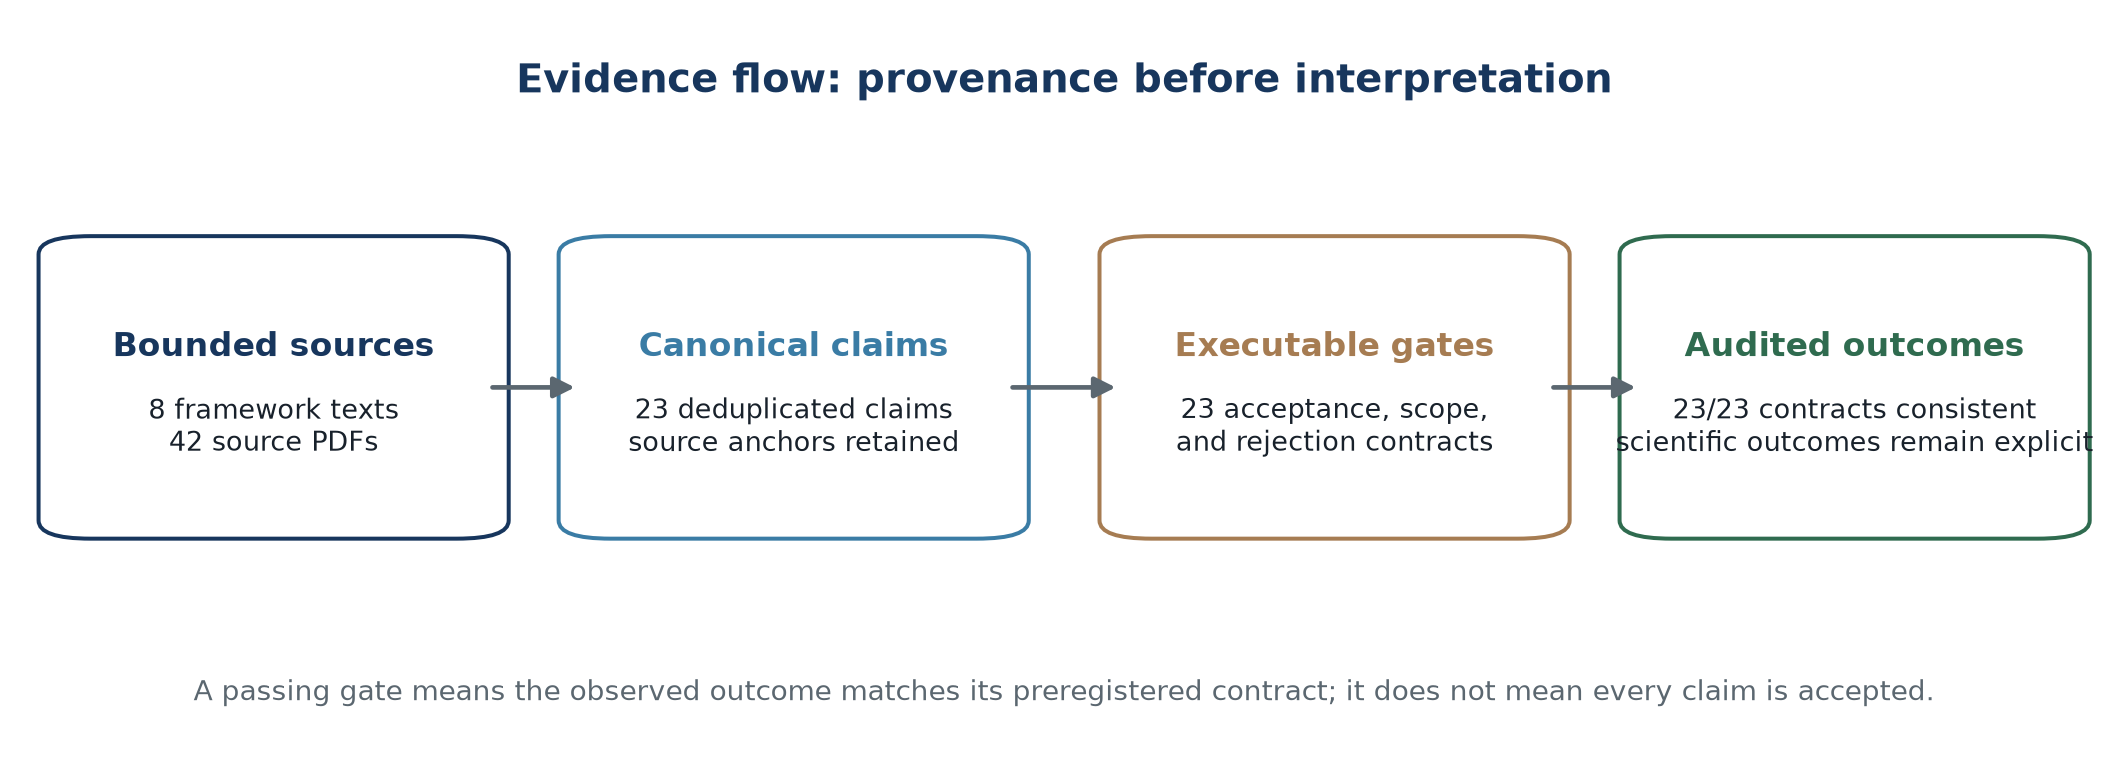
\includegraphics[width=\textwidth]{figures/review_evidence_flow.png}
  \caption{The evidence pipeline separates source provenance, canonical claims,
  executable gates, and admitted conclusions. A passing gate may preserve a
  falsification or exclusion result.}
  \label{fig:evidence-flow}
\end{figure}

\section{Canonical claim disposition}

The unified ledger contains 23 claims. Each has exactly one executable gate,
and the generated result records whether the observed outcome matches the
declared status and rejection contract.

\begin{figure}[htbp]
  \centering
  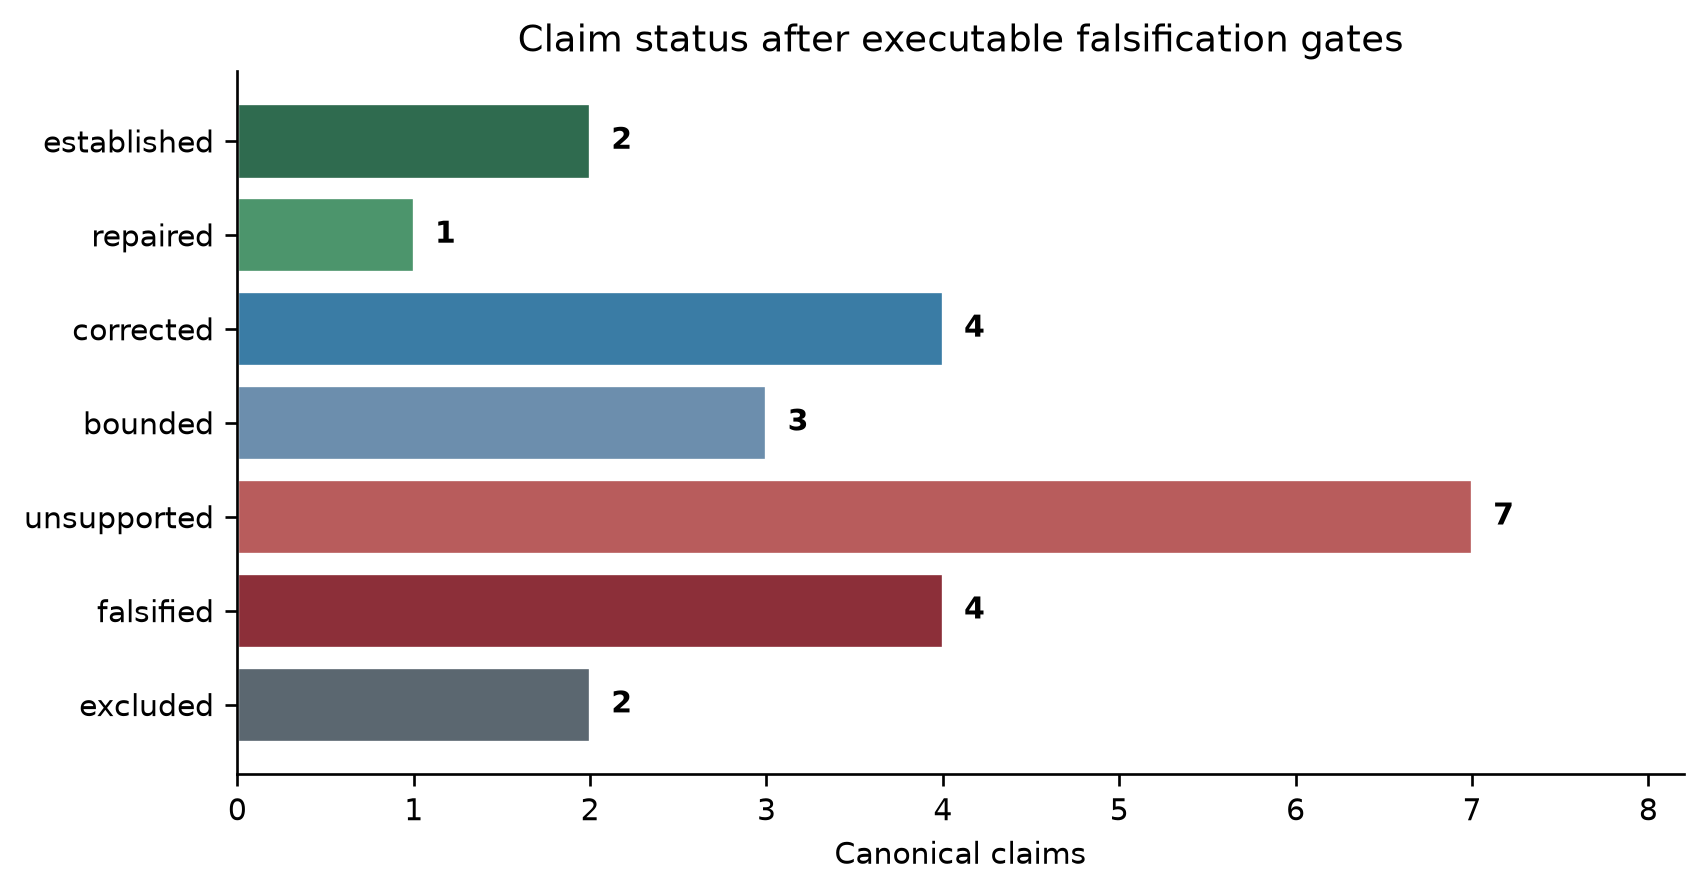
\includegraphics[width=0.82\textwidth]{figures/review_claim_status.png}
  \caption{Claim statuses after mathematical, computational, scope, and
  measurability gates.}
  \label{fig:claim-status}
\end{figure}

\small
\begin{longtable}{>{\raggedright\arraybackslash}p{0.36\textwidth}
                  >{\raggedright\arraybackslash}p{0.16\textwidth}
                  >{\raggedright\arraybackslash}p{0.14\textwidth}
                  >{\raggedright\arraybackslash}p{0.13\textwidth}}
  \caption{Canonical claim status and executable gate outcome.}
  \label{tab:claim-status}\\
  \toprule
  Claim & Domain & Claim status & Gate outcome \\
  \midrule
  \endfirsthead
  \toprule
  Claim & Domain & Claim status & Gate outcome \\
  \midrule
  \endhead
  Octonion normed division boundary & Nonassociative algebra & established & accepted \\
Higher Cayley Dickson physical mapping & Mathematical physics & unsupported & rejected \\
Albert exceptional group ladder & Jordan algebra & corrected & corrected \\
Spin8 triality & Lie theory & established & accepted \\
E9 E10 E11 classification & Kac Moody algebra & corrected & corrected \\
E10 E11 supergravity scope & Quantum gravity & bounded & bounded \\
Monstrous moonshine stability & Modular forms & unsupported & rejected \\
Fractional and negative dimension scope & Fractal geometry & corrected & corrected \\
Fractal estimator convergence & Numerical analysis & bounded & bounded \\
Scalar field curvature mechanism & Field theory & unsupported & rejected \\
ZPE energy harvesting & Quantum field theory & unsupported & rejected \\
Time crystal energy amplification & Condensed matter physics & unsupported & rejected \\
Planck force unification & Dimensional analysis & unsupported & rejected \\
Origami fold merge operator & Operator theory & excluded & excluded \\
E7 root quotient charge & Lattice theory & falsified & falsified \\
External Fourier quotient map & Lattice theory & falsified & falsified \\
Kac Moody fluid transfer & Mathematical physics & unsupported & rejected \\
LBM beta plane and jets & Computational fluid dynamics & falsified & falsified \\
Matched beta plane algebraic ablation & Computational fluid dynamics & falsified & falsified \\
LBM equilibrium conservation & Computational fluid dynamics & repaired & repaired \\
Tourmaline novel energy effect & Materials science & bounded & bounded \\
Gravitoelectromagnetism scope & General relativity & corrected & corrected \\
Consciousness resonance & Biophysics & excluded & excluded \\
\bottomrule

\end{longtable}
\normalsize

\section{Limits of this review}

The review does not independently reproduce every theorem cited in the corpus,
nor does it treat repository tests as substitutes for peer review. It evaluates
what the checked-in artifacts can support. Claims that require laboratory data,
hardware execution, or a new mathematical proof remain open only when the
claim is defined precisely enough to test. Otherwise they remain unsupported,
not merely unfinished.

The beta-plane study is a short, decaying, periodic-domain implementation test;
it does not establish statistically stationary turbulence or persistent jets.
The algebra audits combine literature scope with exact counterexamples and
finite numerical residuals; sampled identities do not replace universal proofs.
No new materials, vacuum-energy, time-crystal-energy, gravitational, or
biophysical experiment was performed. Those claims therefore remain bounded,
rejected, or excluded according to their admission packages rather than being
promoted by the breadth of the source corpus.

\chapter{Falsification of the Critiques}
\label{ch:critique-reassessment}

A critique is itself a claim. This chapter therefore subjects each material
objection from the first audit to the same rule applied to the source corpus:
name a possible falsifier, inspect the relevant repository surface, and retain
only the narrowest verdict supported by the result. A surviving critique is
not strengthened by rhetoric. A failed critique is narrowed or withdrawn.

The canonical record is
\path{data/registry/critique_evidence_ledger.json}. The table below is generated
from that ledger, and generation fails when an evidence path is missing. This
keeps the prose verdict, machine-readable status, and repository evidence on
one truth surface.

\small
\begin{longtable}{>{\raggedright\arraybackslash\bfseries}p{0.22\textwidth}
                  >{\raggedright\arraybackslash}p{0.43\textwidth}
                  >{\raggedright\arraybackslash}p{0.23\textwidth}}
  \caption{Critique-by-critique falsification record.}
  \label{tab:critique-reassessment}\\
  \toprule
  Critique & Falsification attempt and repository evidence & Verdict \\
  \midrule
  \endfirsthead
  \toprule
  Critique & Falsification attempt and repository evidence & Verdict \\
  \midrule
  \endhead
% Generated by scripts/generate_critique_evidence_table.py.
  The value c to the fourth divided by G proves force unification &
    Search the retained sources for field content, a common gauge structure, derived couplings, or a distinguishing prediction. The corpus supplies dimensional identities and interpretations but no such derivation. &
    Survives: The identity defines a force scale, not a unification mechanism. \\
  Cancellation of hbar is independent physical evidence &
    Expand Planck energy divided by Planck length. The cancellation is an algebraic consequence of the selected derived units. &
    Survives: No independent macroscopic quantum effect follows from the cancellation. \\
  E7 roots carry nontrivial P/Q parity &
    Classify all 126 generated roots. Every root belongs to the root lattice Q and therefore represents the zero coset. &
    Survives: The stated root-class map is trivial. \\
  No nontrivial Fourier-to-P/Q map can exist &
    Enumerate every homomorphism from Z\textasciicircum{}2 to the E7 quotient P/Q isomorphic to Z/2 and impose square-lattice D4 symmetry. The unique nontrivial invariant map is h(kx,ky)=(kx+ky) mod 2. &
    Falsified: A nontrivial symmetry-compatible map exists, but homomorphism additivity admits every exact triad and therefore supplies no nontrivial triad filter. \\
  A modular triad filter drives the simulation &
    Search the CPU, JAX, notebook, and high-resolution driver paths for quotient labels and a triad-admission predicate. Neither exists. &
    Survives: The proposed operator is absent from the implemented dynamics. \\
  The retained dynamics implement a beta plane &
    Trace every parameter into collision, forcing, and streaming. The notebook computes a beta value, but beta does not enter the evolution. &
    Survives: Arithmetic after the run is not beta-dependent dynamics. \\
  Root enumeration is nondeterministic &
    Repeat generation across hash seeds and inspect the set-to-array boundary. The tested float tuples were stable, but set iteration was an unstated dependency; the generator now sorts lexicographically. &
    Repaired: Enumeration is deterministic, while physical invariance under ordering remains unproved. \\
  Root order is physically irrelevant &
    Compare the canonical density scaffold with controlled permutations. Reversal is exactly invariant because opposite roots share absolute coordinates, while a one-place cyclic shift changes the perturbation by 0.131 in relative L2. &
    Falsified: One symmetry-related permutation is harmless, but index weighting remains load-bearing. \\
  The high-resolution run has catastrophic mass growth &
    Read all retained Parquet states. Relative drift reaches only 5.60e-6 at step 500. &
    Narrowed: Catastrophic growth belonged to the separate historical CPU demonstration. \\
  The historical CPU demonstration conserves mass &
    Sum the historical D2Q9 equilibrium at nonzero velocity. Its coefficients applied the sound-speed factors twice, producing density times one plus nine times speed squared. &
    Repaired: The historical critique survives, and the current equation and validator now pass conservation tests. \\
  The retained run supports four zonal jets &
    Measure the final state with a fixed diagnostic. Mode 17 dominates the small zonal-mean profile, which is only 1.22e-3 of total velocity RMS; the vorticity moment ratio is 0.992. &
    Survives: A peak index alone does not establish a strong zonal regime. \\
  The reported Rhines comparison is independent &
    Trace beta\_eff in the notebook. It is reconstructed from the observed velocity and peak wavenumber used in the comparison. &
    Survives: The reported agreement is circular. \\
  Affine symmetry transfers to the fluid through the E8 label &
    Search for currents, operator products, a stress tensor, and Ward tests. The repository supplies none. &
    Survives: The Sugawara result does not transfer to the fluid model by naming. \\
  Imaginary algebraic roots are evanescent spatial modes &
    Search for a dimensional map between the Kac-Moody bilinear form and a spatial dispersion relation. None is defined. &
    Survives: The identification conflates different quadratic forms. \\
  The corpus contains no empirical materials evidence &
    Inspect the tourmaline and zero-point-vibration sources. They include ordinary electrical and thermal measurements and standard lattice-vibration calculations. &
    Falsified: Relevant conventional evidence is present. \\
  The corpus supports novel tourmaline or excess-energy effects &
    Search for calibrated raw data, complete energy balances, blinded controls, and independent replication of the proposed enhancement. &
    Survives: Conventional evidence does not test the novel coupling. \\
  Two indexed JSON artifacts are unusable &
    Parse the historical files, identify truncation, and rerun deterministic generators with schema-valid output and invariant tests. &
    Repaired: The historical critique survives; the current artifacts are parseable and regenerated. \\
  Registry inclusion establishes scientific validity &
    Compare identity checks with parsing, schema, conservation, and model gates. Registry identity is necessary but not sufficient. &
    Survives: A digest establishes byte identity, not scientific validity. \\
  The retained fractal dimensions are converged &
    Compare retained estimates with exact controls and inspect scale-window stability. Multiple estimates disagree and no refinement study closes the gap. &
    Survives: The values are finite-resolution diagnostics. \\
  Layered harmonics measure an E7 physical effect &
    Trace the retained schedule to a physical observable or discriminating control. It is a parameter construction without such a link. &
    Survives: The artifact records a chosen construction rather than a measured E7 effect. \\
  A matched dynamical ablation is the uniquely smallest next test &
    Separate zero-cost structural checks from dynamical experiments. Exhaustive triad inventory can reject the proposed filter before any simulation. &
    Falsified: The exhaustive audit closes the homomorphic filter before dynamics; a beta-plane run now serves as a negative matched control rather than a rescue test. \\
  \bottomrule

\end{longtable}
\normalsize

The reassessment changes the paper in three ways. It withdraws absolute claims
about the absence of conventional materials evidence, confines catastrophic
mass growth to the defective historical CPU run, and records repaired artifacts
as current regressions rather than continuing to call them malformed. The main
physical objections survive because the missing maps, operators, and controls
remain missing after those corrections.

\chapter{Mathematical Baseline}
\label{ch:mathematics}

\section{Exceptional and extended Lie algebras}

The finite-dimensional exceptional complex simple Lie algebras are
$G_2$, $F_4$, $E_6$, $E_7$, and $E_8$. Their ranks, dimensions, root counts,
and Cartan matrices are established classification data. The affine and
indefinite extensions commonly denoted $E_9$, $E_{10}$, and $E_{11}$ are
Kac--Moody algebras, not additional members of the finite exceptional list
\citep{kac1990infinite}.

For a simply laced finite root system with root lattice $Q$ and weight lattice
$P$, the finite quotient $P/Q$ has order equal to the determinant of the Cartan
matrix. Thus

\begin{equation}
  |P/Q| = \det A,
  \qquad
  \det A_{E_6}=3,
  \quad
  \det A_{E_7}=2,
  \quad
  \det A_{E_8}=1.
\end{equation}

\begin{evidence}{Established result}
These identities classify lattices and representations. They do not, without
an explicit mode map and dynamics, determine transport coefficients, forcing
amplitudes, jet counts, or material response.
\end{evidence}

The $E_8$ lattice is even and unimodular in eight dimensions, and its minimal
vectors form the 240 roots of $E_8$. The lattice also appears in the solution
of the eight-dimensional sphere-packing problem \citep{cohn2017sphere}. None of
these statements supplies a physical coupling merely by reusing the label
$E_8$ in a simulation.

The exceptional Jordan algebra, or Albert algebra, is the 27-dimensional
algebra $J_3(\OO)$ of Hermitian $3\times3$ octonionic matrices. Its exceptional
group ladder depends on which structure is preserved:

\begin{table}[htbp]
  \centering
  \caption{Corrected exceptional-group roles associated with the Albert algebra.}
  \label{tab:albert-group-ladder}
  \begin{tabular}{lll}
    \toprule
    Group & Dimension & Preserved structure \\
    \midrule
    $F_4$ & 52 & Jordan-algebra automorphisms \\
    $E_{6(-26)}$ & 78 & determinant-preserving reduced structure \\
    $E_{7(-25)}$ & 133 & conformal/Freudenthal structure \\
    \bottomrule
  \end{tabular}
\end{table}

Therefore $E_7$ is not the automorphism group of a putative $J_3(S)$ built
from sedenions. The repository audit now evaluates a nonzero octonionic Jordan
product, verifies its identity and commutativity residuals, tests the Jordan
identity, and records the three distinct group roles. This replaces the former
implementation, whose matrix product returned zero for every input.

\section{Cayley--Dickson algebras}

The Cayley--Dickson construction produces real algebras of dimension $2^n$.
The first four are

\begin{equation}
  \RR,
  \qquad
  \CC,
  \qquad
  \HH,
  \qquad
  \OO.
\end{equation}

Algebraic properties are progressively lost under doubling. In particular,
the sedenions contain zero divisors, so the existence of a high-dimensional
Cayley--Dickson algebra does not make it a division algebra or a viable space
of physical states \citep{baez2001octonions,schafer1954composition}.

\begin{evidence}{Established result with a computational illustration}
A finite program can exhibit a zero-divisor pair or test identities on sampled
elements. Such a run illustrates a known theorem; it neither proves the theorem
nor validates a physical use of the algebra.
\end{evidence}

\scriptsize
\begin{longtable}{lrrrrrrrr}
  \caption{Cayley--Dickson property boundary reproduced by the executable audit.}
  \label{tab:cayley-property-boundary}\\
  \toprule
  Algebra & Dim. & Comm. & Assoc. & Alt. & Power & Flex. & Norm & ZD \\
  \midrule
  \endfirsthead
  \toprule
  Algebra & Dim. & Comm. & Assoc. & Alt. & Power & Flex. & Norm & ZD \\
  \midrule
  \endhead
  Real & 1 & Yes & Yes & Yes & Yes & Yes & Yes & No \\
Complex & 2 & Yes & Yes & Yes & Yes & Yes & Yes & No \\
Quaternion & 4 & No & Yes & Yes & Yes & Yes & Yes & No \\
Octonion & 8 & No & No & Yes & Yes & Yes & Yes & No \\
Sedenion & 16 & No & No & No & Yes & Yes & No & Yes \\
Pathion & 32 & No & No & No & Yes & Yes & No & Yes \\
\bottomrule

\end{longtable}
\normalsize

Here ``Power'' means power-associative, ``Flex.'' means flexible, ``Norm''
means multiplicative norm, and ``ZD'' records a nonzero zero divisor. The exact
sedenion witness is $(e_3+e_{10})(e_6-e_{15})=0$.

\section{Modular forms and moonshine}

A holomorphic modular form of integer weight $k$ for $\mathrm{SL}(2,\ZZ)$
is holomorphic on the upper half-plane, satisfies
$f((a\tau+b)/(c\tau+d))=(c\tau+d)^k f(\tau)$, and is holomorphic
at the cusp. For subgroups, every cusp requires its own boundary condition.
The modular invariant $j$ is a modular function: it has a pole at the cusp. The classical modular invariant has
the expansion

\begin{equation}
  j(\tau) = q^{-1} + 744 + 196884q + 21493760q^2 + \cdots,
  \qquad q=e^{2\pi i\tau}.
\end{equation}

The appearance of Monster-group representation dimensions in coefficients of
$j$ led to monstrous moonshine, proved using the Monster
Lie algebra and its twisted denominator identities \citep{conway1979monstrous,borcherds1992monstrous}.

\begin{evidence}{Established result}
Recomputing a few coefficients or special values checks an implementation.
It does not establish that an unrelated physical system has Monster symmetry.
That requires a defined action, observables transforming under it, and tests
that distinguish the symmetry from alternatives.
\end{evidence}

In particular, the theorem identifies graded Monster traces with specified
genus-zero modular functions. It supplies no generic stability operator for a
fluid, fractal, or material evolution equation. The physical claim is rejected
unless a state space, Monster action, evolution operator, invariant or norm,
stability inequality, and matched non-moonshine control are all defined.

\section{Fractal dimensions}

Hausdorff and box-counting dimensions are well-defined mathematical invariants,
but finite-resolution estimators depend on scale selection, sampling, and
regression choices \citep{falconer2004fractal}. A high coefficient of
determination for a log--log fit is not by itself evidence of asymptotic scaling.
The fitted window must be stable under resolution changes and must avoid the
finite-size and discretization plateaus.

\section{The inference boundary}

The established objects in this chapter can parameterize models. They do not
select a model on their own. A defensible cross-domain construction must provide
all of the following:

\begin{enumerate}
  \item a map from the mathematical object to physical degrees of freedom;
  \item equations of motion that use the mapped structure;
  \item units and normalization for every parameter;
  \item a baseline model without the proposed structure;
  \item an observable that differs between the models; and
  \item uncertainty estimates or a convergence study for the comparison.
\end{enumerate}

Without these items, the mathematics may be correct while the physical
interpretation remains an unsupported extrapolation.

\chapter{Audit of the Physical Claims}
\label{ch:physical-claims}

\section{Planck force and force unification}

The quantity

\begin{equation}
  F_{\mathrm{P}} = \frac{c^4}{G}
\end{equation}

has dimensions of force. It can also be written as the Planck energy divided by
the Planck length. These are algebraic identities among constants and derived
units \citep{planck1899natural}.

\begin{evidence}{Source claim}
The reviewed Superforce manuscript interprets this scale as a force of
unification \citep{pais2023superforce}. The repository reproduces the
dimensional cancellation and the value of the scale.
\end{evidence}

\begin{evidence}{Assessment: unsupported extrapolation}
Dimensional agreement is necessary for an equation but does not derive an
interaction. A force-unification claim requires a field content, symmetry,
couplings, renormalization behavior, and predictions that differ from general
relativity and the Standard Model. None follows from $c^4/G$ alone. Substituting
Planck units into Newtonian or Coulomb force laws selects a scale; it does not
show that distinct gauge interactions become the same mechanism.
\end{evidence}

The absence of $\hbar$ from $c^4/G$ also has no independent physical content:
$\hbar$ cancels in the ratio of two Planck units. The cancellation cannot, by
itself, establish a macroscopic quantum effect.

\section{Root-lattice charges and fluid triads}

The earlier manuscript proposed that Fourier modes inherit a class in the
discriminant group $P/Q$ and that triad closure conserves those classes. The
proposal fails at its first stated map. If the forcing vectors are roots, then
they lie in the root lattice $Q$ and every root represents the zero class in
$P/Q$. The proposed nontrivial parity charge therefore does not arise from the
root set as written.

A nontrivial construction would need, at minimum:

\begin{enumerate}
  \item a homomorphism from the physical Fourier lattice to $P/Q$;
  \item a reason physical modes occupy nonzero weight-lattice cosets;
  \item a forcing or interaction operator that enforces the proposed charge;
  \item a count of admitted and rejected triads under that operator; and
  \item a control forcing with matched spectrum, power, and anisotropy but no
    quotient structure.
\end{enumerate}

\begin{evidence}{Assessment: mechanism not implemented}
The repository contains prose describing a modular filter, but the simulation
step contains no $P/Q$ labels and no triad-admission test. The discriminant-group
argument cannot explain a numerical result until that missing map and operator
exist.
\end{evidence}

\section{The beta-plane interpretation}

The Rhines scale follows from competition between turbulent advection and
Rossby-wave dynamics on a beta plane \citep{rhines1975waves,vallis1993generation}.
A beta-plane simulation therefore needs a beta-dependent term in its dynamical
equations, not merely a spectrum that can be assigned a preferred wavenumber
after the run.

The checked-in LBM parameter object has no beta parameter. Its CPU step performs
equilibrium evaluation, BGK collision, streaming, and macroscopic update. The
accelerated step adds a spatially varying relaxation time and random noise, but
no beta-plane body force or potential-vorticity gradient. The high-resolution
driver sets grid size, time steps, relaxation time, and harmonic amplitude.
It does not configure beta.

The implementation selects the first $N$ roots and weights their absolute first
two coordinates by enumeration index. Root generation now uses a deterministic
lexicographic order, removing a reproducibility defect. Determinism does not
make the construction Weyl invariant. The retained order audit finds that
reversal is exactly invariant because lexicographic reversal pairs opposite
roots with equal absolute coordinates, while a one-place cyclic shift changes
the initialized perturbation by 0.131 in relative $L^2$. Any observed
anisotropy remains confounded with this ordering choice, projection, and index
weighting until a symmetry-invariant map and matched controls remove those
alternatives.

The earlier diagnostic

\begin{equation}
  \beta_{\mathrm{inferred}} = U_{\star} k_{\mathrm{jet}}^2
\end{equation}

is useful only after a beta-plane model and an independently defined velocity
scale exist. Choosing or reconstructing $U_{\star}$ from the same output and
then declaring agreement with an asserted beta is circular.

The retained final high-resolution snapshot also contradicts the published
numbers in the superseded assembly. A direct read of the step-500 snapshot gives
a mean speed near $6.92\times10^{-3}$, a maximum speed near
$1.10\times10^{-2}$, and dominant zonal-mean Fourier mode 17. The zonal-mean
RMS is only $8.75\times10^{-6}$, or $1.22\times10^{-3}$ of total velocity RMS,
and the vorticity spectral second-moment ratio is 0.992. Thus the selected peak
mode is not evidence of a strong zonal state. The earlier text used
$U\approx0.6$ and mode 4. The run driver does not compute a jet count, spectral
slope, or uncertainty interval, so those earlier values have no traceable
analysis path.

\begin{table}[htbp]
  \centering
  \caption{Requirements for a defensible beta-plane comparison.}
  \label{tab:beta-requirements}
  \begin{tabularx}{\textwidth}{>{\raggedright\arraybackslash\bfseries}p{0.28\textwidth}YY}
    \toprule
    Requirement & Repository state & Consequence \\
    \midrule
    Beta-dependent dynamics & Absent from the retained LBM steps & The run is not a beta-plane experiment. \\
    Independent input beta & No beta field in the parameter object & Input-output agreement cannot be tested. \\
    Prespecified jet diagnostic & Not retained with uncertainty or mode-selection rule & Jet count is post hoc. \\
    Matched controls & No isotropic or spectrum-matched ablation & Algebraic causation is unidentified. \\
    Conservation check & JAX drift is $5.60\times10^{-6}$ at step 500; the repaired CPU regression is conservative & Catastrophic growth does not describe the high-resolution run. \\
    \bottomrule
  \end{tabularx}
\end{table}

\section{Affine algebras and conformal invariance}

For an affine Lie algebra at level $k$, the Sugawara construction produces a
Virasoro action under specified representation-theoretic conditions. For
affine $E_8$ at level one, the central charge is

\begin{equation}
  c = \frac{k\,\dim E_8}{k+h^{\vee}} = \frac{248}{31}=8.
\end{equation}

This is a statement about a current algebra and its conformal field theory. It
does not imply that a fluid forced with a pattern labelled $E_8$ inherits that
Virasoro representation. Two-dimensional turbulence can display conformal
statistics in appropriate regimes \citep{bernard2006conformal}, but similarity
of vocabulary is not a derivation.

\begin{evidence}{Assessment: category error}
Persistent homology can summarize geometry in data. It cannot prove that a
fluid field carries a Sugawara stress tensor. The latter requires an explicit
current algebra, operator products or equivalent observables, and Ward-identity
tests.
\end{evidence}

\section{Imaginary roots and evanescent waves}

An imaginary root of an indefinite Kac--Moody algebra is defined by the root
space bilinear form. It is not an imaginary spatial wavenumber. Identifying the
two square roots without a map between the bilinear forms conflates algebraic
classification with a dispersion relation. The repository supplies no such
map, so the proposed \enquote{evanescent threshold} and \enquote{superforce
limit} are unsupported.

\section{Gravitoelectromagnetism}

Gravitoelectromagnetism is a controlled analogy inside general relativity, not
a direct coupling between electromagnetic and gravitational fields. In the
linear perturbation construction, a Minkowski background is perturbed by
$h_{\mu\nu}$, the trace-reversed perturbation obeys a sourced wave equation
after a transverse gauge condition is imposed, and the gravitoelectric and
gravitomagnetic fields are defined from the resulting potentials
\citep{mashhoon2008gravitoelectromagnetism}. The Lorentz-like test-body form is
therefore conditional on the weak-field expansion, the stated gauge and source
definitions, and the retained velocity order.

The analogy does not create a new electromagnetic--gravitational coupling,
does not replace the nonlinear Einstein equations, and does not establish a
propulsion mechanism. A stronger claim requires a covariant action with the
proposed interaction, consistent source and test-body variables, recovery of
the general-relativistic limit, and a controlled prediction that ordinary
electromagnetic coupling, vibration, and thermal drift do not explain.

\section{Materials and zero-point-energy claims}

The repository retains manuscripts concerning tourmaline, vibrations, and
zero-point-energy interpretations. The corpus includes conventional empirical
material data, including tourmaline electrical and thermal measurements, and
standard first-principles calculations of zero-point vibration. This evidence
falsifies an absolute claim that the source collection is wholly nonempirical.
It does not test the proposed enhancement, excess-energy effect, or new
coupling. Those claims require calibrated raw measurements, a complete energy
balance, blinded controls, uncertainty budgets, and independent replication.
The checked-in corpus contains no such discriminating evidence.

The experimental-admission registry converts that boundary into operational
packages. Measurable proposals receive observables, matched controls, complete
energy channels, acceptance criteria, and rejection criteria. Undefined
analogies receive no pretend observable and remain excluded.

\begin{table}[htbp]
  \centering
  \caption{Operational content of the physical-claim admission packages.}
  \label{tab:experimental-admission-packages}
  \small
  \begin{tabularx}{\textwidth}{>{\raggedright\arraybackslash}p{0.43\textwidth}Yrrrr}
    \toprule
    Claim & Outcome & Obs. & Ctrls. & Channels & Missing \\
    \midrule
    Scalar field curvature mechanism & rejected & 3 & 3 & 6 & 4 \\
ZPE energy harvesting & rejected & 3 & 3 & 8 & 4 \\
Time crystal energy amplification & rejected & 3 & 3 & 9 & 4 \\
Tourmaline novel energy effect & bounded & 3 & 3 & 9 & 4 \\
Origami fold merge operator & excluded & 0 & 0 & 0 & 4 \\
Consciousness resonance & excluded & 0 & 0 & 0 & 4 \\
\bottomrule

  \end{tabularx}
\end{table}

\chapter{Computational Evidence Portfolio}
\label{ch:computation}

\section{Selection and evaluation rule}

This chapter reviews eight retained artifact families. Each entry records the
method, the paper-ready output it could support, one validation check, and the
strongest permissible inference. This format prevents an implementation check
from silently becoming a claim about nature.

\small
\begin{longtable}{>{\raggedright\arraybackslash}p{0.14\textwidth}
                  >{\raggedright\arraybackslash}p{0.26\textwidth}
                  >{\raggedright\arraybackslash}p{0.23\textwidth}
                  >{\raggedright\arraybackslash}p{0.20\textwidth}}
  \caption{Experiment artifacts, figure targets, and validation gates.}
  \label{tab:experiment-portfolio}\\
  \toprule
  Artifact & Method and figure target & Validation check & Permissible inference \\
  \midrule
  \endfirsthead
  \toprule
  Artifact & Method and figure target & Validation check & Permissible inference \\
  \midrule
  \endhead
  Fractal estimates &
    \path{experiments/results/fractal_dimensions.json}. Finite-resolution box
    counting or correlation sums. Plot fitted slope by
    scale with the selected window marked. &
    Repeat at increasing sample counts and shift the fit window. Compare with
    known dimensions. &
    Tests the estimator on selected synthetic sets. \\
  Modular forms &
    \path{experiments/results/modular_forms_analysis.json}. Truncated series
    evaluation. Plot absolute error for known special values
    against truncation order. &
    Verify $j(i)=1728$ and the zero at the cubic elliptic point to stated
    tolerance. &
    Checks numerical evaluation of standard identities. \\
  Cayley--Dickson &
    \path{experiments/results/cayley_dickson_real_validation.json}. Generated
    property record. A table reports finite identity checks by dimension. &
    Regenerate atomically, parse as JSON, and compare checks with direct
    calculations. &
    Finite computational checks of standard algebraic properties. \\
  E8 analysis &
    \path{experiments/results/e8_analysis.json}. Generated root-system summary.
    Plot root norms and pairwise inner-product
    multiplicities. &
    Parse the file, then test root count, rank, norms, opposite closure, and
    Cartan determinant against independent construction. &
    Finite validation of the generated $E_8$ root corpus. \\
  High-resolution LBM Parquet snapshots &
    BGK-style lattice-Boltzmann evolution with noise. Plot mass, momentum, and
    kinetic energy versus step before any spectrum. &
    Inspect schemas, prove fixed boundary and forcing conventions, and bound
    conservation drift. &
    Retained numerical trajectories, not beta-plane evidence. \\
  LBM demonstration &
    \path{experiments/quantum_lbm_stable_results.json}. A 32 by 32, 50-step
    conservation regression. Plot total mass and kinetic energy versus step. &
    Require relative mass drift below a prespecified tolerance. &
    The corrected CPU path conserves mass; it remains a numerical test, not
    evidence of quantum or exceptional-algebra dynamics. \\
  Layered harmonics &
    \path{experiments/data/genesis_harmonics_e7.json}. Deterministic layered
    frequencies and amplitudes. Plot amplitude against
    layer index with the generating formula. &
    Regenerate byte-equivalent output from a recorded version and seed. &
    Describes a chosen parameterization; it does not measure E7 physics. \\
  Generated registries &
    File discovery, size, and SHA-256 capture. Plot artifact counts by kind or
    use a compact inventory table. &
    Rebuild registries and verify every digest and schema. &
    Supports provenance and integrity only. \\
  \bottomrule
\end{longtable}

\section{Repaired result serialization}

The first audit found two experiment JSON files truncated inside scalar values.
That historical failure showed that registry inclusion checked identity but not
parseability. The current files are generated by
\path{scripts/generate_core_validation_results.py}, written atomically, parsed
by tests, and checked against explicit finite invariants. The E8 record now
contains 240 roots, 120 positive roots, rank 8, dimension 248, norm-squared
multiplicity 240 at value 2, opposite closure, and Cartan determinant 1. The
Cayley--Dickson record reports only properties actually calculated by its
generator.

\begin{evidence}{Repaired computational artifacts}
The files now support their stated finite checks. Repairing serialization does
not promote those checks into physical evidence, and future registry generation
still needs a general parse-and-schema gate rather than file existence alone.
\end{evidence}

\section{Fractal-dimension estimates}

The retained fractal result contains scales, measures, fitted dimensions,
regression errors, and coefficients of determination. This is a better evidence
shape than a single scalar. It still lacks a convergence study over resolution
and fit-window selection. For example, the retained Cantor-set estimate is
approximately $0.675$, while the exact middle-thirds value is
$\log 2/\log 3\approx0.631$. The discrepancy is large enough that the estimator
must be described as finite-resolution and method-dependent.

\begin{evidence}{Computational check}
The artifact can support a methods figure showing scale dependence. It cannot
support a claim that arbitrary framework geometries have a validated fractal
dimension.
\end{evidence}

\section{Modular-form special values}

The modular-form artifact records $j(i)=1728$ numerically and a near-zero value
at an approximation to the cubic elliptic point. It also records initial
coefficients of the $j$ expansion and Ramanujan tau values. These are useful
regression targets because independent reference values exist.

\begin{evidence}{Computational check}
Agreement verifies a limited numerical implementation. The computation contains
no data from a physical system and therefore supplies no evidence for a
moonshine-based physical mechanism.
\end{evidence}

\section{The CPU LBM defect and repair}

The first audit found that the file named
\texttt{quantum\_lbm\_stable\_results.json} grew from initial mass near
$1.024\times10^3$ to final mass near $1.251\times10^6$ after 50 steps. The
failure was not generic LBM instability. The CPU equilibrium used standard
D2Q9 coefficients and then divided by the sound-speed powers a second time.
At nonzero velocity its populations summed to $\rho(1+9|u|^2)$ rather than
$\rho$.

The equilibrium now uses the dimensionally consistent coefficient form. The
conservation validator measures relative error against initialized mass instead
of returning a constant verdict. The regenerated 50-step periodic run conserves
mass to approximately $1.78\times10^{-15}$ relative error. Tests also inject
mass deliberately and require the validator to reject the altered state.

\begin{evidence}{Repaired numerical regression}
The corrected result validates one conservation prerequisite for the CPU code.
The root-indexed initial condition and passive auxiliary arrays still supply no
evidence for quantum transport, coherent flow, or a cross-domain physical map.
\end{evidence}

\section{High-resolution snapshot mismatch}

The high-resolution driver leaves the requested harmonic count and Reynolds
metadata unchanged, giving 127 and 100 respectively. Only 126 E7 roots exist,
so the effective initializer count is 126; the Reynolds field does not enter
the evolution. The superseded paper assembly instead reported 10 harmonics and
Reynolds number 10. A direct read of the final Parquet snapshot
finds dominant zonal-mean mode 17, mean speed $6.92\times10^{-3}$, and maximum
speed $1.10\times10^{-2}$, not the published mode 4 and characteristic speed
0.6. The mode-17 zonal profile is weak: its RMS is $1.22\times10^{-3}$ of total
velocity RMS. A vorticity-power second-moment ratio of 0.992 is close to
isotropic. Relative mass drift rises smoothly to $5.60\times10^{-6}$ by step
500; this is measurable but not the catastrophic CPU failure. No checked-in
analysis computes the reported uncertainty or a $-5/3$ fit.

\begin{evidence}{Retained output contradicts the superseded claim}
Every reported table cell must be generated from a versioned analysis command
and stored beside the run parameters. Values that cannot be traced to that path
are removed rather than rounded into agreement.
\end{evidence}

\section{Resolved structural gate and controlled next experiment}

The exhaustive triad inventory closes the structural gate. The unique
nontrivial square-symmetry-invariant homomorphism from the Fourier lattice to
$P/Q\simeq\mathbb{Z}/2$ is $h(k_x,k_y)=k_x+k_y\pmod 2$. It admits every exact
triad by additivity, so the proposed filter equals its identity control before
any dynamics are run.

The short matched beta-plane ablation tests implementation sensitivity and
records the algebraic filter as a prespecified negative control. It is not the
scientific jet test. The production program separately executes 540 paired
runs across five beta values, three drag values, three viscosities, and twelve
independent seed clusters:

\begin{enumerate}
  \item implement the beta-dependent evolution independently of quotient labels;
  \item compare the homomorphic filter with its bit-identical identity control;
  \item specify mass, energy, enstrophy, anisotropy, and jet diagnostics before
    running;
  \item execute a committed-before-rerun resolution and time-step refinement study;
  \item report seed-clustered effect sizes and simultaneous uncertainty bounds;
  \item require zero filter effect to numerical precision and reject any claimed
    algebraic effect if the trajectories differ.
\end{enumerate}

The numerical, refinement, and control gates pass. The registered scientific
hypothesis does not. At $\beta=5$, the zonal-fraction effect is $-0.0030$ and
the persistent-jet-prevalence effect is $0.1019$. At $\beta=10$, the effects
are $-0.0200$ and $0.0000$. Every required simultaneous interval crosses zero,
and every required effect misses its locked minimum. An independent clean
container reproduces the negative aggregate decision. The result is evidence
against the declared transient-zonalization effect in this freely decaying
model; it is not evidence against beta-plane jet formation under other forcing
or dissipation regimes.

This experiment cannot rehabilitate the root-lattice interpretation. The first
nonhomomorphic candidate also fails specificity: its $E_7$ quadratic-defect
mask is exactly the generic even-checkerboard kernel at every enumerated triad.
Generic parity-kernel dynamics would define a different mechanism and still
requires conservation and matched-control gates.

\begin{figure}[htbp]
  \centering
  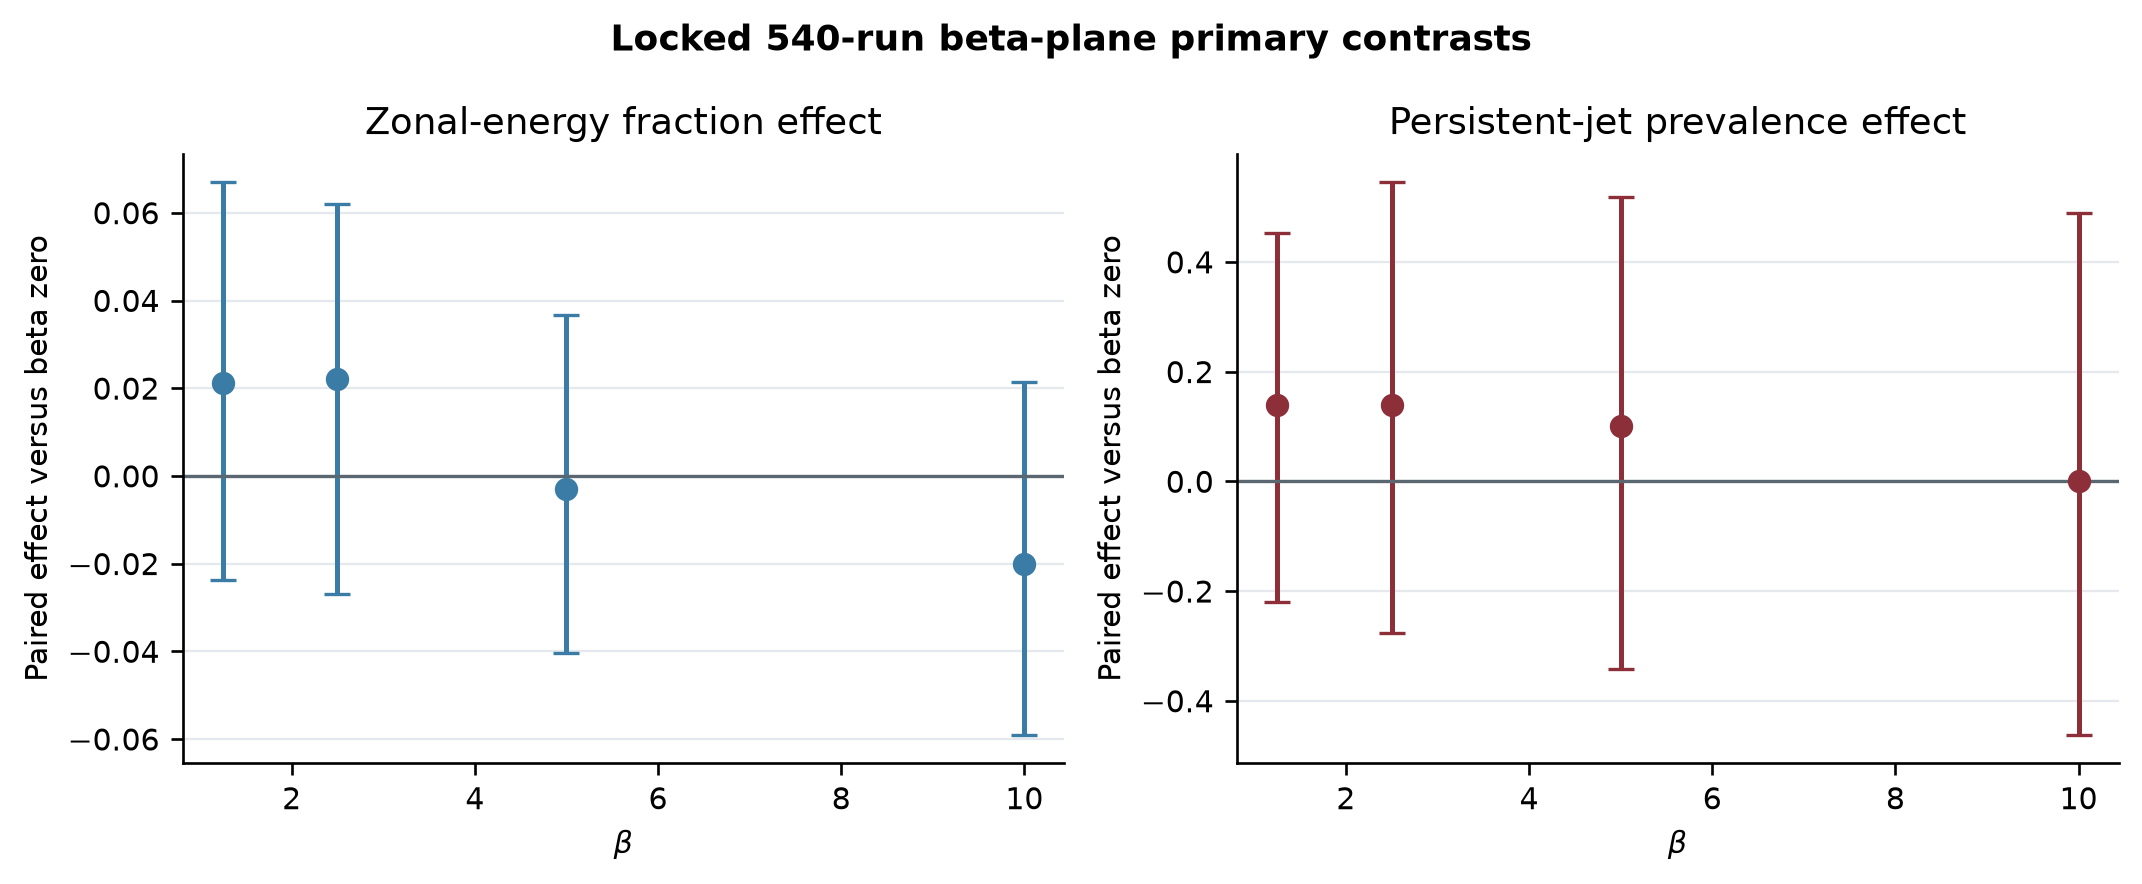
\includegraphics[width=\textwidth]{figures/review_beta_ablation.png}
  \caption{Primary effects from the locked 540-run beta-plane matrix. Error
  bars are simultaneous familywise 95 percent bootstrap intervals over twelve
  seed clusters. None of the four required $\beta=5,10$ contrasts passes.}
  \label{fig:beta-ablation}
\end{figure}

\begin{table}[htbp]
  \centering
  \caption{Required contrasts from the locked beta-plane production matrix.}
  \label{tab:beta-ablation-results}
  \small
  \begin{tabularx}{\textwidth}{>{\raggedright\arraybackslash}p{0.29\textwidth}YYYY}
    \toprule
    Metric & Effect & Lower bound & Upper bound & Decision \\
    \midrule
    Zonal-energy fraction at $\beta=5$ & -0.0030 & -0.0404 & 0.0368 & Not supported \\
Persistent-jet prevalence at $\beta=5$ & 0.1019 & -0.3426 & 0.5185 & Not supported \\
Zonal-energy fraction at $\beta=10$ & -0.0200 & -0.0592 & 0.0215 & Not supported \\
Persistent-jet prevalence at $\beta=10$ & 0.0000 & -0.4630 & 0.4885 & Not supported \\
\bottomrule

  \end{tabularx}
\end{table}

\chapter{Reconciled Framework Architecture}
\label{ch:framework-reconciliation}

\section{Why concatenation is not integration}

The retained framework corpus contains eight text files, but they are not eight
independent theories. A deterministic paragraph audit finds that
\texttt{Alpha001.06} and \texttt{Maximal Extraction} contain the same 390
unique normalized blocks. The former repeats these blocks until 2,078 eligible
block occurrences remain, of which 1,688 are internal duplicates. Counting
these repetitions as agreement would turn copying into evidence.

The consolidation therefore preserves the original documents as archival
sources and constructs a new framework from unique claims. Exact duplicate
spans collapse to one canonical statement with multiple provenance aliases.
Similar headings nominate a semantic review; they do not authorize merging
different equations or physical mechanisms.

\begin{figure}[htbp]
  \centering
  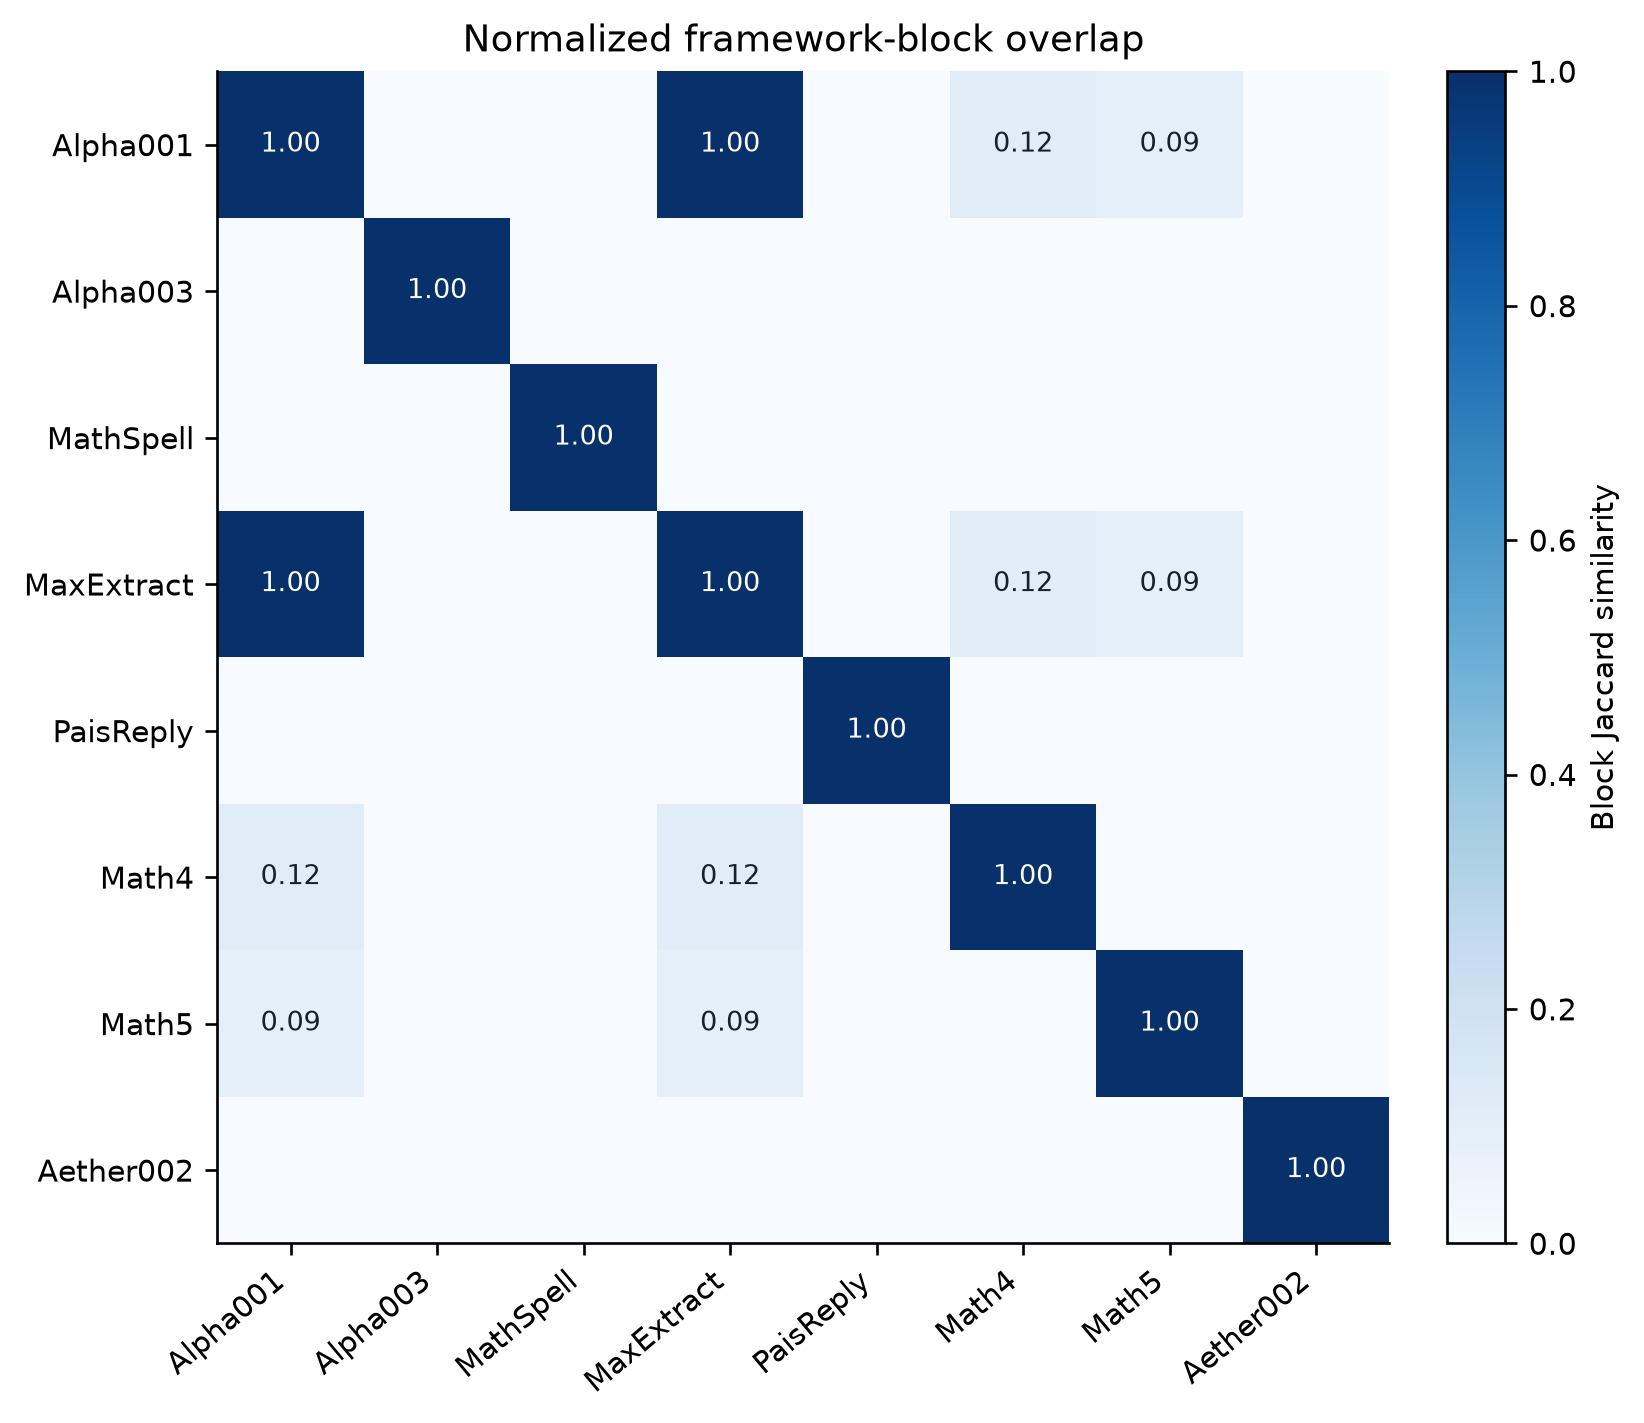
\includegraphics[width=0.82\textwidth]{figures/review_framework_overlap.png}
  \caption{Exact normalized-block overlap among the eight retained framework
  documents. The unit overlap identifies duplicate lineage rather than
  independent corroboration.}
  \label{fig:framework-overlap}
\end{figure}

\section{One framework, five evidence layers}

The unified framework is organized by evidential role rather than source order.

\begin{description}
  \item[Defined mathematics] Octonions, higher Cayley--Dickson algebras,
    exceptional and Kac--Moody algebras, the Albert algebra, lattices, modular
    forms, spectral geometry, and named notions of dimension enter with their
    standard definitions and known boundaries.
  \item[Typed bridges] A cross-domain map must name its source object, target
    object, map, preserved invariants, assumptions, and observable.
  \item[Reproducible computation] Code enters only after schema, determinism,
    invariant, refinement, and control gates appropriate to its claim.
  \item[Physical hypotheses] A proposed mechanism must descend from a defined
    action, Hamiltonian, constitutive law, or stochastic process and must state
    units, parameters, observables, and a null model.
  \item[Historical ideation] Undefined analogies and nonempirical claims remain
    traceable but do not enter the scientific core.
\end{description}

This architecture preserves productive conjectures without allowing them to
inherit theorem-level confidence from the mathematical objects they mention.

\section{Resolved mathematical conflicts}

\subsection{Cayley--Dickson scope}

The real normed division algebras stop at the octonions
\citep{baez2001octonions}. Higher Cayley--Dickson doublings remain legitimate
algebraic objects, and their zero divisors are mathematically structured
\citep{moreno2005constructing}; however, division, norm composition, and other
identities cannot be assumed to persist. A proposed physical application must
identify the exact multiplication law, subspace, invariant, and observable it
uses. Dimension alone supplies no mechanism.

\subsection{Albert algebra and exceptional groups}

The source statement that $E_6$ is the automorphism group of
$J_3(\mathbb{O})$ and $E_7$ the automorphism group of a sedenionic
$J_3(\mathbb{S})$ is rejected. The Albert algebra is built from octonions;
$F_4$ is its automorphism group, while suitable forms of $E_6$ and $E_7$ arise
as structure and conformal groups \citep{baez2001octonions}. These group
actions are different objects,
not interchangeable meanings of \enquote{symmetry}.

\subsection{The E-series boundary}

$E_6$, $E_7$, and $E_8$ are finite-dimensional exceptional simple Lie
algebras. $E_9$, $E_{10}$, and $E_{11}$ are affine, hyperbolic, and
very-extended Kac--Moody structures. Restricted supergravity dictionaries
motivate research programs \citep{damour2002e10,west2001e11}; they do not prove
a complete symmetry of observed interactions.

\section{Resolved physical boundaries}

\subsection{Time crystals}

The equilibrium continuous-time-crystal proposal is excluded under broad
conditions by the Watanabe--Oshikawa no-go theorem
\citep{watanabe2015absence}. Floquet time crystals are instead driven
nonequilibrium many-body phases \citep{else2016floquet}, and primary experiments
observe their subharmonic response \citep{zhang2017observation}. The drive,
dissipation, and finite lifetime remain part of the energy budget. These results
do not supply free amplification of vacuum energy.

\subsection{Vacuum response and energy extraction}

Casimir forces do not by themselves prove that zero-point energy is an
extractable reservoir \citep{jaffe2005casimir}. Dynamical-Casimir photon
production uses work supplied through a driven boundary condition
\citep{wilson2011observation}. Quantum energy inequalities further constrain
negative-energy magnitude and duration \citep{fewster2012lectures}. A proposed
device must close its complete energy balance over a cycle before an excess-
energy claim enters the framework.

\subsection{Planck force and unification}

The quantity $c^4/G$ is a force scale. The cancellation of $\hbar$ in a ratio
of derived Planck units is an algebraic identity, not independent physical
evidence. A unification claim still requires field content, a common action,
coupling relations, correct low-energy limits, and a distinguishing prediction.

\section{Open hypotheses with admission gates}

The root-to-$P/Q$ charge proposal is falsified because every root lies in the
root lattice and therefore represents the zero coset. An external map can be
defined: the unique nontrivial square-symmetry-invariant homomorphism is
$h(k_x,k_y)=k_x+k_y\pmod 2$. It still cannot filter exact convolution triads,
because $k+p+q=0$ implies $h(k)+h(p)+h(q)=0$. The map-existence question is
closed positively and the homomorphic filter mechanism is closed negatively.

The historical fluid evolution contains no beta term and its retained final
state is nearly isotropic under fixed diagnostics. The new preregistered
barotropic solver includes the beta term and passes budget, refinement, and
multi-seed implementation gates. Its homomorphic quotient-filter arm is exactly
identical to the identity arm. The short decaying ablation establishes
implementation sensitivity only. The separate 540-run production matrix does
not support the registered transient-zonalization conjunction; its four
required contrasts and simultaneous intervals appear in
\cref{tab:beta-ablation-results}.

A scalar-gravity hypothesis requires a covariant action, stress-energy tensor,
background solution, perturbation equations, stability criterion, and an
observable distinguishable from an ordinary scalar-tensor model. The generic
sourced scalar equation in the drafts does not satisfy this contract.

\section{Durable authority}

The machine-readable authority is
\path{data/registry/unified_framework_claims.json}. It records canonical
statements, original source anchors, status, confidence, literature and
repository evidence, falsification tests, and integration actions. The
human-readable framework is
\path{docs/framework/UNIFIED_EVIDENCE_FRAMEWORK.md}. Unsupported ideas can be
reformulated, but a changed claim receives a new identifier rather than erasing
the failed version.

% Hypothesis registry and promotion policy

\chapter{Hypothesis Registry and Promotion Gates}
\label{ch:hypothesis-registry}

The claim ledger and the hypothesis registry serve different purposes. A claim
contract checks whether the repository's stated disposition agrees with its
retained evidence. It does not turn a rejected or unsupported claim into a
successful experiment. The hypothesis registry instead records the formal
replacement statement, observable prediction, controls, falsification
threshold, required evidence, implementation state, and reproduction state for
every bounded, unsupported, excluded, or falsified canonical claim.

The registry contains 14 atomic hypotheses covering 16 canonical source claims.
It also dispositions 54 explicit prompts from dormant legacy chapters as
mapped, superseded, field-level open problems, or excluded because they are
undefined. These archival items are not part of the manuscript's active claim
surface. Their retention prevents an old prediction table or open-problem list
from silently restoring a claim that the evidence review has already bounded.

\section{Promotion rule}

A supported or negative computational or empirical result enters the paper
only after all of the following conditions hold:

\begin{enumerate}
  \item the hypothesis and its controls are registered before the production
    run;
  \item the implementation passes its numerical and structural gates;
  \item the locked decision rule is evaluated without endpoint substitution;
  \item a supported claim passes every registered acceptance threshold, while
    a negative claim reports exactly which component or conjunction fails and
    does not convert non-support into component-wise exclusion;
  \item a cache-isolated pinned environment repeats the decision without
    reusing the primary run cache;
  \item the reproduction record retains the source commit, environment image
    digest, preregistration digest, primary and reproduction result digests,
    command, reviewer, and evidence paths; and
  \item the hypothesis registry marks the result eligible or promoted.
\end{enumerate}

The same evidence may support a negative conclusion without supporting the
proposed mechanism. Exact checkerboard equality falsifies the registered
$E_7$-specificity statement. The beta-plane evidence instead rejects the
registered conjunction as not supported; it does not exclude every component
effect in isolation.

\section{Bounded research programs}

\begin{table}[htbp]
  \centering
  \small
  \begin{tabularx}{\textwidth}{>{\raggedright\arraybackslash}p{0.20\textwidth}>{\raggedright\arraybackslash}p{0.24\textwidth}X}
    \toprule
    Program & Present state & Promotion boundary \\
    \midrule
    Fourier triad selectors & Specificity falsified; reproduced & The failed $P/Q$
      homomorphism remains a negative control. The quadratic-defect mask is the
      generic even-checkerboard kernel. Any parity-kernel experiment still
      requires conservation, matched-mask, and reproduction gates. \\
    Decaying beta-plane flow & Repeated negative result & The 540-run matrix,
      controls, and clean rerun agree on the not-supported decision. The result
      is limited to the registered freely decaying model. \\
    Physical admission & Four operator packages specified & Every physical
      claim remains blocked by calibration, raw measurements, energy or
      constraint closure, blinded controls, and independent replication. \\
    \bottomrule
  \end{tabularx}
  \caption{The three active research programs and the evidence boundary that
  prevents premature manuscript promotion.}
  \label{tab:hypothesis-programs}
\end{table}

The program distinction is substantive. The current barotropic model is
freely decaying and has no forcing operator or injection-energy budget.
Literature on forced--dissipative jet formation constrains interpretation but
does not convert this solver into a sustained-jet experiment
\cite{bakas2015s3t,bakas2019weakjets,sahoo2025interfaces}. Exact and
quasi-resonant Rossby-triad work motivates equation-derived selector controls
without licensing an exceptional-algebra attribution
\cite{kartashov2013rossby,hayat2018rossby}. Similarly, the
$E_7$ discriminant form is established mathematics, whereas imposing its
quadratic defect as a fluid interaction law is a new conjecture that must beat
generic matched masks before any $E_7$ attribution is possible.

No program passes a positive mechanism claim at this revision. The two
cache-isolated negative decisions enter the paper with distinct scopes: exact
equality falsifies $E_7$ specificity, while the beta-plane conjunction is not
supported. Neither result becomes evidence for an alternative exceptional-
algebra mechanism or for beta-plane behavior outside the registered freely
decaying domain. The manuscript otherwise retains the audited mathematical
corrections, exact counterexamples, implementation repairs, and explicit
physical-evidence boundaries.

\registeredresult{hyp_e7_nonhomomorphic_fourier_selector}
\registeredresult{hyp_beta_plane_transient_zonalization}

\chapter{Conclusions and Decision Record}
\label{ch:conclusions}

\section{What survives the audit}

The repository contains useful mathematical and engineering work when its
claims are kept at the scale of the evidence:

\begin{itemize}
  \item standard exceptional-Lie-algebra invariants provide strong regression
    targets for implementations;
  \item Cayley--Dickson computations can illustrate identity loss and zero
    divisors in finite cases;
  \item modular-form special values and series coefficients provide independent
    numerical checks;
  \item fractal estimators retain enough intermediate data to support a proper
    scale-window and convergence analysis;
  \item conventional tourmaline measurements and standard zero-point-vibration
    calculations provide relevant materials context, although not evidence for
    the proposed enhancement; and
  \item registries and digests provide a useful provenance layer for source and
    result artifacts.
\end{itemize}

These are defensible contributions. They do not need a unified-field narrative
to be valuable.

\section{What does not survive}

The central cross-domain conclusions are not established by the checked-in
artifacts:

\begin{itemize}
  \item $c^4/G$ is a force scale, not a derivation of force unification;
  \item root vectors have trivial class in $P/Q$, so the stated discriminant
    selection rule is vacuous, and the separately defined homomorphic Fourier
    map admits every exact triad;
  \item the retained LBM dynamics contain no beta-plane term, so they cannot
    validate a beta-plane interpretation;
  \item a Sugawara construction for an affine algebra does not transfer to a
    fluid field through naming or geometric resemblance;
  \item imaginary algebraic roots are not imaginary spatial wavenumbers; and
  \item repairing JSON serialization and CPU mass conservation does not supply
    the missing physical map, beta dynamics, or matched controls.
\end{itemize}

\section{Strongest defensible interpretation}

The compendium is best understood as a software-backed review environment for
testing mathematical implementations and auditing speculative source claims.
It is not evidence for a unified physical framework. The repository becomes
more useful when a failed test is allowed to remain a failed test and when a
correct identity is not asked to carry a causal conclusion it does not imply.

\section{Integrated evidence architecture}

The review now enforces one directional chain of authority:

\begin{enumerate}
  \item retained source bytes establish what the reviewed documents contain;
  \item native text, MinerU decomposition, and Tesseract fallback provide
    separately hashed representations of those bytes;
  \item the critique ledger binds each objection to a falsification attempt,
    a controlled verdict vocabulary, and concrete evidence paths;
  \item deterministic generators and numerical tests establish finite
    mathematical or computational properties;
  \item schema and digest gates establish that registries describe the live
    artifacts rather than stale predecessors; and
  \item the manuscript states only the narrowest conclusion licensed by all
    upstream gates.
\end{enumerate}

No downstream layer can promote an upstream result to a stronger evidence
class. Better OCR cannot turn a source claim into a measurement. A matching
digest cannot turn a malformed model into a valid one. A conservative solver
cannot supply a missing physical map. The integration is valuable precisely
because each component constrains the others instead of lending them borrowed
authority.

\section{Resolved conjectures and remaining hypotheses}

Two initially open conjectures now have negative mechanism results. The unique
nontrivial square-symmetry-invariant Fourier homomorphism to $E_7$'s
$P/Q\simeq\mathbb{Z}/2$ exists, but additivity admits every exact convolution
triad. In the matched beta-plane ablation, beta changes every trajectory while
the quotient-filter arm remains exactly identical to the identity arm. The
historical four-jet conclusion and the revised algebraic-filter explanation are
therefore both falsified for their stated implementations.

The remaining physical proposals are not one undifferentiated conjectural
framework. The scalar-curvature, vacuum-harvesting, time-crystal-amplification,
and tourmaline-novelty packages each define distinct observables, controls,
energy channels, and rejection rules. None is admission-ready because the
required raw evidence is absent. Fold-merge and consciousness-resonance claims
remain excluded because they do not define operational variables. Any revised
mechanism receives a new claim identifier and must pass its own gate.

\section{Publication gate}

A future edition may advance a new physical mechanism only when all of the
following are present:

\begin{enumerate}
  \item a complete mathematical definition with typed domains and codomains;
  \item a derivation connecting that definition to the implemented equations;
  \item a reproducible parameter manifest and parseable result schema;
  \item numerical conservation and convergence checks;
  \item matched controls or ablations that isolate the claimed mechanism;
  \item uncertainty estimates across seeds or experimental replicates; and
  \item a falsification criterion fixed before inspecting the result.
\end{enumerate}

The correct immediate outcome is therefore not a stronger unification claim.
It is a smaller, testable claim and an experiment capable of returning no.


\appendix
\chapter{Reproducibility and Artifact Inventory}
\label{app:reproducibility}

\section{Build the manuscript}

From the repository root, run:

\begin{verbatim}
make papers
\end{verbatim}

The clean-checkout sequence is:

\begin{verbatim}
make document-ocr-generate
make document-decomposition-index
\end{verbatim}

OCR outputs remain generated local caches under \path{build/document_ocr/}.
The retained run manifest records the container image ID, pinned base image,
exact commands, modes, and output roots. The decomposition registry records the
hashes needed to compare a regenerated cache with the reviewed run.

The paper build uses the checked-in bibliography and regenerates the
registry-driven evidence figures and result tables. The broader scientific and
interactive figure suite remains a separate target because it requires the full
Python environment and may alter unrelated generated artifacts.

The beta-plane and selector results use a separate pinned clean-room image:

\begin{verbatim}
EVIDENCE_SOURCE_COMMIT=$(git rev-parse HEAD)
tools/reproduction/build_exact_source_image.sh \
  "$EVIDENCE_SOURCE_COMMIT"
EVIDENCE_SOURCE_COMMIT="$EVIDENCE_SOURCE_COMMIT" \
  docker compose -f tools/reproduction/compose.yaml run --rm
EVIDENCE_SOURCE_COMMIT="$EVIDENCE_SOURCE_COMMIT" \
  make validate-clean-reproduction
\end{verbatim}

The builder exports the declared commit with \texttt{git archive}; uncommitted
host files never enter the build context. The image pins its base by OCI digest,
installs the repository lock file, and records a digest manifest for every
source-tree file after installation.
The reproduction service receives no primary build cache. It writes a separate
production result, refinement result, control result, selector audit, raw-array
archives, run log, environment report, and host-side image identity under
\path{data/reproduction/}. The clean-reproduction verifier compares the source
files inside the image with the declared Git tree, validates the environment
manifest, and compares normalized results and raw archives with the primary
run. Promotion validation recomputes every declared digest and rejects a
reproduction whose runner and reviewer identities match.

\section{Decompose the source documents}

The source corpus contains 42 PDFs and 1,076 pages. Embedded text is retained as
one evidence layer, not assumed to be correct. The page-level audit routes
sparse pages for OCR:

\begin{verbatim}
python3 scripts/audit_pdf_text_quality.py
\end{verbatim}

Formula- and layout-aware extraction uses the pinned MinerU 3.4.4 CUDA image in
high-effort hybrid mode:

\begin{verbatim}
docker compose -f tools/document_ocr/compose.yaml build mineru
docker compose -f tools/document_ocr/compose.yaml run --rm mineru \
  'mineru -p /workspace/source_materials/pdfs \
    -o /workspace/build/document_ocr/mineru_corpus \
    -b hybrid-engine --effort high -m auto \
    --formula true --table true --image-analysis true'
\end{verbatim}

Tesseract 5 is an independent fallback, not the primary parser:

\begin{verbatim}
python3 scripts/run_tesseract_pdf_ocr.py \
  source_materials/pdfs/Comment_on_the_Pais_Superforce_Theory.pdf
\end{verbatim}

On the sparse 13-page Superforce commentary, MinerU recovers structured
headings, display mathematics, reading order, diagrams, and image regions.
Tesseract recovers useful prose but degrades several equations. Native text,
MinerU, and Tesseract outputs remain separate so later review can trace which
representation supports a quotation or formula.

\section{Run the repository quality gates}

The relevant commands are:

\begin{verbatim}
make papers
make test
make lint
make verify-offline
\end{verbatim}

\texttt{make lint-latex} checks generated critique evidence, unresolved stubs,
and ASCII source hygiene. \texttt{make papers} additionally rebuilds the PDF
and fails on unresolved references, duplicate labels, margin overflow,
malformed bibliography entries, and build warnings. Python and registry gates
remain separate so a missing optional runtime cannot masquerade as success.

\section{Evidence-bearing artifacts}

\begin{table}[htbp]
  \centering
  \small
  \caption{Primary repository evidence surfaces used in this review.}
  \label{tab:evidence-surfaces}
  \begin{tabularx}{\textwidth}{p{0.34\textwidth}X}
    \toprule
    Path & Role \\
    \midrule
    \path{source_materials/pdfs/} & Retained source documents. \\
    \path{papers/references.bib} & Bibliographic metadata used by this manuscript. \\
    \path{src/mathphysics/} & Reusable mathematical and numerical implementations. \\
    \path{experiments/} & Drivers and retained experiment outputs. \\
    \path{results/} & Parquet simulation snapshots. \\
    \path{data/registry/artifacts_index.toml} & Generated artifact identities and digests. \\
    \path{data/registry/experiments_index.toml} & Generated experiment-output inventory. \\
    \path{data/registry/parquet_audit.json} & Schema-inspection status for retained snapshots. \\
    \path{data/registry/lbm_evidence_audit.json} & Generated conservation, velocity, zonal, and anisotropy diagnostics. \\
    \path{data/registry/lbm_root_order_audit.json} & Controlled sensitivity of the root-indexed initializer to ordering. \\
    \path{data/evidence/beta_plane/} & Deterministic primary production, refinement, and control-array archives. \\
    \path{data/reproduction/} & Independent clean-container results, raw arrays, environment record, and logs. \\
    \path{data/registry/independent_reproduction_registry.json} & Digest-bound promotion decisions for supported and negative results. \\
    \path{data/registry/critique_evidence_ledger.json} & Canonical status, falsification attempt, verdict, and evidence paths for all 21 critiques. \\
    \path{data/registry/pdf_text_quality_audit.json} & Page-level embedded-text quality and OCR routing. \\
    \path{data/registry/document_decomposition_audit.json} & MinerU output hashes and artifact counts for all 42 PDFs and 1,076 pages. \\
    \path{data/registry/document_ocr_run_manifest.json} & MinerU container identity, exact modes and commands, and Tesseract manifest identity. \\
    \path{data/registry/pdf_ocr_comparison.json} & Native, MinerU, and Tesseract comparison for the sparsest document. \\
    \path{data/registry/pdf_ocr_visual_review.json} & Retained page-level equation, layout, diagram, and prose comparison rubric. \\
    \path{data/registry/claim_source_crosswalk.toml} & Source lineage for selected claims. \\
    \bottomrule
  \end{tabularx}
\end{table}

\section{Artifact validity rules}

An artifact enters a scientific argument only if it passes all applicable
checks:

\begin{enumerate}
  \item the file parses according to its declared format;
  \item its schema includes units, parameters, and version or commit identity;
  \item its digest matches the generated registry;
  \item the producing command is recorded and succeeds from a clean environment;
  \item prerequisite invariants, including conservation or normalization, pass;
  \item the analysis method and selection rules are specified before the result;
  \item the claimed inference does not exceed what the artifact measures.
\end{enumerate}

Checksums satisfy only the third item. A registry should not label an artifact
scientifically valid merely because it exists and hashes reproducibly.

\section{Current limitations and blockers}

At the time of this review, serialization, CPU mass conservation, deterministic
root enumeration, Cartan construction, Albert multiplication, PDF
decomposition, and Parquet schema inspection have been repaired. The structural
Fourier map and matched beta-plane questions have executable negative results.
The remaining scientific blockers are:

\begin{itemize}
  \item the historical high-resolution LBM driver has no beta-plane parameter
    or term and remains evidence only for its own nearly isotropic trajectory;
  \item the homomorphic Fourier-to-$P/Q$ mechanism is closed negatively, and
    the first nonhomomorphic candidate is exactly a generic checkerboard kernel;
  \item the high-resolution states lack a complete retained parameter and
    software-version manifest;
  \item the reported four-jet and $-5/3$ conclusions have no traceable analysis;
    and
  \item the 540-run freely decaying beta-plane matrix does not support its
    registered transient-zonalization effect outside the tested domain; and
  \item scalar gravity, ZPE harvesting, time-crystal amplification, and
    tourmaline novelty lack the raw measurements required by their operational
    admission packages.
\end{itemize}

These blockers are evidence, not housekeeping. They determine which claims the
manuscript can honestly make.


\backmatter
\chapter*{Declarations}
\addcontentsline{toc}{chapter}{Declarations}

\textbf{Document type.} This work is a repository-backed review monograph. A
venue-specific journal template is outside the evidence claim and must not
change the registered results.

\textbf{Author contributions.} Eirikr Hinngart curated the source corpus,
implemented the audits and experiments, reviewed the evidence, and prepared
the manuscript. Automated tools assisted code generation, OCR, testing, and
adversarial review; their activity remains attributable through the repository
history and does not constitute authorship.

\textbf{Data and code availability.} Source, code, registries, and retained
evidence are available at
\url{https://github.com/Oichkatzelesfrettschen/MathScienceCompendium}. The
pre-experiment evidence baseline is tag \texttt{v0.1.0-evidence}. Exact source,
container, protocol, result, archive, and verification digests for the promoted
negative results are recorded in
\path{data/registry/independent_reproduction_registry.json}.

\textbf{Competing interests.} The author declares no competing interests in
the claims evaluated in this review.

\textbf{Ethics.} This review reports no new human-participant or animal study.

\bibliographystyle{plainnat}
\bibliography{references}

\end{document}
